\documentclass{ieeeaccess}
\usepackage{cite}
\usepackage{amsmath,amssymb,amsfonts}
\usepackage{algorithmic}
\usepackage{graphicx}
\usepackage{textcomp}
\def\BibTeX{{\rm B\kern-.05em{\sc i\kern-.025em b}\kern-.08em
    T\kern-.1667em\lower.7ex\hbox{E}\kern-.125emX}}
\begin{document}
\history{Date of publication xxxx 00, 0000, date of current version xxxx 00, 0000.}
\doi{10.1109/ACCESS.2017.DOI}

\title{Belief rule base inference method based on gradient descent with momentum}
\author{\uppercase{First A. Author}\authorrefmark{1}, \IEEEmembership{Fellow, IEEE},
    \uppercase{Second B. Author\authorrefmark{2}, and Third C. Author,
        Jr}.\authorrefmark{3},
    \IEEEmembership{Member, IEEE}}
\address[1]{National Institute of Standards and
    Technology, Boulder, CO 80305 USA (e-mail: author@boulder.nist.gov)}
\address[2]{Department of Physics, Colorado State University, Fort Collins,
    CO 80523 USA (e-mail: author@lamar.colostate.edu)}
\address[3]{Electrical Engineering Department, University of Colorado, Boulder, CO
    80309 USA}
\tfootnote{This paragraph of the first footnote will contain support
    information, including sponsor and financial support acknowledgment. For
    example, ``This work was supported in part by the U.S. Department of
    Commerce under Grant BS123456.''}

\markboth
{Author \headeretal: Preparation of Papers for IEEE TRANSACTIONS and JOURNALS}
{Author \headeretal: Preparation of Papers for IEEE TRANSACTIONS and JOURNALS}

\corresp{Corresponding author: First A. Author (e-mail: author@ boulder.nist.gov).}

\begin{abstract}

    The belief-rule-base(BRB) inference methodology using evidential reasonging(ER)
    approach is widely used in different fields, such as  fault diagnosis, system
    identification and decision analysis.
    In this paper, we propose a new belief rule structure and its training method,
    aiming to solve zero activation during the inference process and improve inference accuray.
    We first used the Gaussian function to calculate the similarity of each attribute instead of the original method.
    Then we introduce corresponding attribute weight for each rule and cancel the rule weight parameter at the same time.
    Finally, we use the stochastic gradient descent method for parameters training based on the new rule structure.
    Experiments on several public classification datasets are conducted to validate the proposed approach compared with some recent existing works.
    The experimental results show that the proposed approach have a better performence in accuray and time consumption.

\end{abstract}

\begin{keywords}
    belief rule base, structure optimization, stochastic gradient descent, momentum optimization.
\end{keywords}

\titlepgskip=-15pt

\maketitle

\section{Introduction}
\label{sec:introduction}

The belief rule-based inference methodology using evidential reasonging approach(RIMER) proposed by Yang\cite{a1}
baesd on traditional IF-THEN rules\cite{a2}, Dempster-Shafer theory of evidence\cite{a3,a4}, decision theory\cite{a5}
and fuzzy set theory\cite{a6}. By introducing a belief distribution structure in the rules, this methodology can
effectively handle incomplete and uncertain information involved in the datasets and widely used in various problem in
different fields such as oil pipeline leak detection\cite{a7}, military capability estimation\cite{a8}, consumer behavior
prediction\cite{a9} and so on.

In the inference process of the BRB system, the attribute weight, rule weight, belief distribution and other parameters
directly affect the final accuray. Yang\cite{a10} proposed optimization models for training BRB system using fmincon solver in
Matlab, Chang\cite{a11,a12} proposed an algorithm for training parameters in BRB system based on gradient and dichotomy methods,
Wu\cite{a13} used the accelerating of gradient algorithm to improve the convergence accuray and convergence speed. There are also
a series of intelligent algorithms such as the particle swarm algorithm proposed by Su\cite{a14} and the differential evolution
algorithm proposed by Wang\cite{a15} have excellent training effects on the BRB system. Liu\cite{a16} introduces the belief distribution
structure into the antecedent attributes and uses training data to build an extended belief rule base(EBRB) system, which simplifies the construction of
the rule base and improves the inference speed.

At present, the parameter optimization model of the BRB system is mostly based on various intelligent algorithms. Their process is
complicated and there are many intermediate training parameters. When the traditional gradient method is used to train the parameters
of the BRB system, the step size is restricted by a variety of constraints, and other methods are needed to find the optimal step size.
The EBRB system does not introduce a parameter training process, which makes the system have higher requirements for the representativeness
of the training data selected to build the rule base. In the case of a large number of rules, it is necessary to perform rule reduction or
use the data structure to optimize the storage and activation process of the rules. Because the traditional BRB system includes the rule attribute
reference level setting, its potential zero activation problem may cause the inference system to fail.

In response to the above problems, we have proposed a series of optimization modifications to the system structure and reasoning process, including:

\quad 1) We propose a new antecedent structure that does not need to set the attribute reference level, and proposed a Gaussian function-based
rule weight activation method for the new rule antecedent structure, which can effectively avoid the zero activation problem and has the feature of
generating rules from the training data like EBRB.

\quad 2) We change the method of setting the weight of the global same antecedent attribute in the
traditional BRB system, and set the corresponding rule attribute weight parameter for each rule, so that each rule has a finer activation granularity.
On this basis, the rule weight and its related normalization process are cancelled, which simplifies the evidential reasoning process.

\quad 3) We further introduce the linear rectification function and the normalized exponential function to preprocess the restricted parameters to avoid the problem of
parameter failure during the parameter training process.



\section{Units}
Use either SI (MKS) or CGS as primary units. (SI units are strongly
encouraged.) English units may be used as secondary units (in parentheses).
This applies to papers in data storage. For example, write ``15
Gb/cm$^{2}$ (100 Gb/in$^{2})$.'' An exception is when
English units are used as identifiers in trade, such as ``3\textonehalf-in
disk drive.'' Avoid combining SI and CGS units, such as current in amperes
and magnetic field in oersteds. This often leads to confusion because
equations do not balance dimensionally. If you must use mixed units, clearly
state the units for each quantity in an equation.

The SI unit for magnetic field strength $H$ is A/m. However, if you wish to use
units of T, either refer to magnetic flux density $B$ or magnetic field
strength symbolized as $\mu _{0}H$. Use the center dot to separate
compound units, e.g., ``A$\cdot $m$^{2}$.''

\section{Some Common Mistakes}
The word ``data'' is plural, not singular. The subscript for the
permeability of vacuum $\mu _{0}$ is zero, not a lowercase letter
``o.'' The term for residual magnetization is ``remanence''; the adjective
is ``remanent''; do not write ``remnance'' or ``remnant.'' Use the word
``micrometer'' instead of ``micron.'' A graph within a graph is an
``inset,'' not an ``insert.'' The word ``alternatively'' is preferred to the
word ``alternately'' (unless you really mean something that alternates). Use
the word ``whereas'' instead of ``while'' (unless you are referring to
simultaneous events). Do not use the word ``essentially'' to mean
``approximately'' or ``effectively.'' Do not use the word ``issue'' as a
euphemism for ``problem.'' When compositions are not specified, separate
chemical symbols by en-dashes; for example, ``NiMn'' indicates the
intermetallic compound Ni$_{0.5}$Mn$_{0.5}$ whereas
``Ni--Mn'' indicates an alloy of some composition
Ni$_{x}$Mn$_{1-x}$.

\Figure[t!](topskip=0pt, botskip=0pt, midskip=0pt){fig1.png}
{Magnetization as a function of applied field.
    It is good practice to explain the significance of the figure in the caption.\label{fig1}}

Be aware of the different meanings of the homophones ``affect'' (usually a
verb) and ``effect'' (usually a noun), ``complement'' and ``compliment,''
``discreet'' and ``discrete,'' ``principal'' (e.g., ``principal
investigator'') and ``principle'' (e.g., ``principle of measurement''). Do
not confuse ``imply'' and ``infer.''

Prefixes such as ``non,'' ``sub,'' ``micro,'' ``multi,'' and ``ultra'' are
not independent words; they should be joined to the words they modify,
usually without a hyphen. There is no period after the ``et'' in the Latin
abbreviation ``\emph{et al.}'' (it is also italicized). The abbreviation ``i.e.,'' means
``that is,'' and the abbreviation ``e.g.,'' means ``for example'' (these
abbreviations are not italicized).

A general IEEE styleguide is available at \underline{http://www.ieee.org/}\break\underline{authortools}.

\section{Guidelines for Graphics Preparation and Submission}
\label{sec:guidelines}

\subsection{Types of Graphics}
The following list outlines the different types of graphics published in
IEEE journals. They are categorized based on their construction, and use of
color/shades of gray:

\subsubsection{Color/Grayscale figures}
{Figures that are meant to appear in color, or shades of black/gray. Such
    figures may include photographs, illustrations, multicolor graphs, and
    flowcharts.}

\subsubsection{Line Art figures}
{Figures that are composed of only black lines and shapes. These figures
    should have no shades or half-tones of gray, only black and white.}

\subsubsection{Author photos}
{Head and shoulders shots of authors that appear at the end of our papers. }

\subsubsection{Tables}
{Data charts which are typically black and white, but sometimes include
    color.}

\begin{table}
    \caption{Units for Magnetic Properties}
    \label{table}
    \setlength{\tabcolsep}{3pt}
    \begin{tabular}{|p{25pt}|p{75pt}|p{115pt}|}
        \hline
        Symbol                                         &
        Quantity                                       &
        Conversion from Gaussian and \par CGS EMU to SI $^{\mathrm{a}}$                 \\
        \hline
        $\Phi $                                        &
        magnetic flux                                  &
        1 Mx $\to  10^{-8}$ Wb $= 10^{-8}$ V$\cdot $s                                   \\
        $B$                                            &
        magnetic flux density, \par magnetic induction &
        1 G $\to  10^{-4}$ T $= 10^{-4}$ Wb/m$^{2}$                                     \\
        $H$                                            &
        magnetic field strength                        &
        1 Oe $\to  10^{3}/(4\pi )$ A/m                                                  \\
        $m$                                            &
        magnetic moment                                &
        1 erg/G $=$ 1 emu \par $\to 10^{-3}$ A$\cdot $m$^{2} = 10^{-3}$ J/T             \\
        $M$                                            &
        magnetization                                  &
        1 erg/(G$\cdot $cm$^{3}) =$ 1 emu/cm$^{3}$ \par $\to 10^{3}$ A/m                \\
        4$\pi M$                                       &
        magnetization                                  &
        1 G $\to  10^{3}/(4\pi )$ A/m                                                   \\
        $\sigma $                                      &
        specific magnetization                         &
        1 erg/(G$\cdot $g) $=$ 1 emu/g $\to $ 1 A$\cdot $m$^{2}$/kg                     \\
        $j$                                            &
        magnetic dipole \par moment                    &
        1 erg/G $=$ 1 emu \par $\to 4\pi \times  10^{-10}$ Wb$\cdot $m                  \\
        $J$                                            &
        magnetic polarization                          &
        1 erg/(G$\cdot $cm$^{3}) =$ 1 emu/cm$^{3}$ \par $\to 4\pi \times  10^{-4}$ T    \\
        $\chi , \kappa $                               &
        susceptibility                                 &
        1 $\to  4\pi $                                                                  \\
        $\chi_{\rho }$                                 &
        mass susceptibility                            &
        1 cm$^{3}$/g $\to  4\pi \times  10^{-3}$ m$^{3}$/kg                             \\
        $\mu $                                         &
        permeability                                   &
        1 $\to  4\pi \times  10^{-7}$ H/m \par $= 4\pi \times  10^{-7}$ Wb/(A$\cdot $m) \\
        $\mu_{r}$                                      &
        relative permeability                          &
        $\mu \to \mu_{r}$                                                               \\
        $w, W$                                         &
        energy density                                 &
        1 erg/cm$^{3} \to  10^{-1}$ J/m$^{3}$                                           \\
        $N, D$                                         &
        demagnetizing factor                           &
        1 $\to  1/(4\pi )$                                                              \\
        \hline
        \multicolumn{3}{p{251pt}}{Vertical lines are optional in tables. Statements that serve as captions for
        the entire table do not need footnote letters. }                                \\
        \multicolumn{3}{p{251pt}}{$^{\mathrm{a}}$Gaussian units are the same as cg emu for magnetostatics; Mx
            $=$ maxwell, G $=$ gauss, Oe $=$ oersted; Wb $=$ weber, V $=$ volt, s $=$
            second, T $=$ tesla, m $=$ meter, A $=$ ampere, J $=$ joule, kg $=$
            kilogram, H $=$ henry.}
    \end{tabular}
    \label{tab1}
\end{table}

\subsection{Multipart figures}
Figures compiled of more than one sub-figure presented side-by-side, or
stacked. If a multipart figure is made up of multiple figure
types (one part is lineart, and another is grayscale or color) the figure
should meet the stricter guidelines.

\subsection{File Formats For Graphics}\label{formats}
Format and save your graphics using a suitable graphics processing program
that will allow you to create the images as PostScript (PS), Encapsulated
PostScript (.EPS), Tagged Image File Format (.TIFF), Portable Document
Format (.PDF), Portable Network Graphics (.PNG), or Metapost (.MPS), sizes them, and adjusts
the resolution settings. When
submitting your final paper, your graphics should all be submitted
individually in one of these formats along with the manuscript.

\subsection{Sizing of Graphics}
Most charts, graphs, and tables are one column wide (3.5 inches/88
millimeters/21 picas) or page wide (7.16 inches/181 millimeters/43
picas). The maximum depth a graphic can be is 8.5 inches (216 millimeters/54
picas). When choosing the depth of a graphic, please allow space for a
caption. Figures can be sized between column and page widths if the author
chooses, however it is recommended that figures are not sized less than
column width unless when necessary.

There is currently one publication with column measurements that do not
coincide with those listed above. Proceedings of the IEEE has a column
measurement of 3.25 inches (82.5 millimeters/19.5 picas).

The final printed size of author photographs is exactly
1 inch wide by 1.25 inches tall (25.4 millimeters$\,\times\,$31.75 millimeters/6
picas$\,\times\,$7.5 picas). Author photos printed in editorials measure 1.59 inches
wide by 2 inches tall (40 millimeters$\,\times\,$50 millimeters/9.5 picas$\,\times\,$12
picas).

\subsection{Resolution }
The proper resolution of your figures will depend on the type of figure it
is as defined in the ``Types of Figures'' section. Author photographs,
color, and grayscale figures should be at least 300dpi. Line art, including
tables should be a minimum of 600dpi.

\subsection{Vector Art}
In order to preserve the figures' integrity across multiple computer
platforms, we accept files in the following formats: .EPS/.PDF/.PS. All
fonts must be embedded or text converted to outlines in order to achieve the
best-quality results.

\subsection{Color Space}
The term color space refers to the entire sum of colors that can be
represented within the said medium. For our purposes, the three main color
spaces are Grayscale, RGB (red/green/blue) and CMYK
(cyan/magenta/yellow/black). RGB is generally used with on-screen graphics,
whereas CMYK is used for printing purposes.

All color figures should be generated in RGB or CMYK color space. Grayscale
images should be submitted in Grayscale color space. Line art may be
provided in grayscale OR bitmap colorspace. Note that ``bitmap colorspace''
and ``bitmap file format'' are not the same thing. When bitmap color space
is selected, .TIF/.TIFF/.PNG are the recommended file formats.

\subsection{Accepted Fonts Within Figures}
When preparing your graphics IEEE suggests that you use of one of the
following Open Type fonts: Times New Roman, Helvetica, Arial, Cambria, and
Symbol. If you are supplying EPS, PS, or PDF files all fonts must be
embedded. Some fonts may only be native to your operating system; without
the fonts embedded, parts of the graphic may be distorted or missing.

A safe option when finalizing your figures is to strip out the fonts before
you save the files, creating ``outline'' type. This converts fonts to
artwork what will appear uniformly on any screen.

\subsection{Using Labels Within Figures}

\subsubsection{Figure Axis labels }
Figure axis labels are often a source of confusion. Use words rather than
symbols. As an example, write the quantity ``Magnetization,'' or
``Magnetization M,'' not just ``M.'' Put units in parentheses. Do not label
axes only with units. As in Fig. 1, for example, write ``Magnetization
(A/m)'' or ``Magnetization (A$\cdot$m$^{-1}$),'' not just ``A/m.'' Do not label axes with a ratio of quantities and
units. For example, write ``Temperature (K),'' not ``Temperature/K.''

Multipliers can be especially confusing. Write ``Magnetization (kA/m)'' or
``Magnetization (10$^{3}$ A/m).'' Do not write ``Magnetization
(A/m)$\,\times\,$1000'' because the reader would not know whether the top
axis label in Fig. 1 meant 16000 A/m or 0.016 A/m. Figure labels should be
legible, approximately 8 to 10 point type.

\subsubsection{Subfigure Labels in Multipart Figures and Tables}
Multipart figures should be combined and labeled before final submission.
Labels should appear centered below each subfigure in 8 point Times New
Roman font in the format of (a) (b) (c).

\subsection{File Naming}
Figures (line artwork or photographs) should be named starting with the
first 5 letters of the author's last name. The next characters in the
filename should be the number that represents the sequential
location of this image in your article. For example, in author
``Anderson's'' paper, the first three figures would be named ander1.tif,
ander2.tif, and ander3.ps.

Tables should contain only the body of the table (not the caption) and
should be named similarly to figures, except that `.t' is inserted
in-between the author's name and the table number. For example, author
Anderson's first three tables would be named ander.t1.tif, ander.t2.ps,
ander.t3.eps.

Author photographs should be named using the first five characters of the
pictured author's last name. For example, four author photographs for a
paper may be named: oppen.ps, moshc.tif, chen.eps, and duran.pdf.

If two authors or more have the same last name, their first initial(s) can
be substituted for the fifth, fourth, third$\ldots$ letters of their surname
until the degree where there is differentiation. For example, two authors
Michael and Monica Oppenheimer's photos would be named oppmi.tif, and
oppmo.eps.

\subsection{Referencing a Figure or Table Within Your Paper}
When referencing your figures and tables within your paper, use the
abbreviation ``Fig.'' even at the beginning of a sentence. Do not abbreviate
``Table.'' Tables should be numbered with Roman Numerals.

\subsection{Checking Your Figures: The IEEE Graphics Analyzer}
The IEEE Graphics Analyzer enables authors to pre-screen their graphics for
compliance with IEEE Access standards before submission.
The online tool, located at
\underline{http://graphicsqc.ieee.org/}, allows authors to
upload their graphics in order to check that each file is the correct file
format, resolution, size and colorspace; that no fonts are missing or
corrupt; that figures are not compiled in layers or have transparency, and
that they are named according to the IEEE Access naming
convention. At the end of this automated process, authors are provided with
a detailed report on each graphic within the web applet, as well as by
email.

For more information on using the Graphics Analyzer or any other graphics
related topic, contact the IEEE Graphics Help Desk by e-mail at
graphics@ieee.org.

\subsection{Submitting Your Graphics}
Because IEEE will do the final formatting of your paper,
you do not need to position figures and tables at the top and bottom of each
column. In fact, all figures, figure captions, and tables can be placed at
the end of your paper. In addition to, or even in lieu of submitting figures
within your final manuscript, figures should be submitted individually,
separate from the manuscript in one of the file formats listed above in
Section \ref{formats}. Place figure captions below the figures; place table titles
above the tables. Please do not include captions as part of the figures, or
put them in ``text boxes'' linked to the figures. Also, do not place borders
around the outside of your figures.

\subsection{Color Processing/Printing in IEEE Journals}
All IEEE Transactions, Journals, and Letters allow an author to publish
color figures on IEEE Xplore\textregistered\ at no charge, and automatically
convert them to grayscale for print versions. In most journals, figures and
tables may alternatively be printed in color if an author chooses to do so.
Please note that this service comes at an extra expense to the author. If
you intend to have print color graphics, include a note with your final
paper indicating which figures or tables you would like to be handled that
way, and stating that you are willing to pay the additional fee.

\section{Conclusion}
A conclusion section is not required. Although a conclusion may review the
main points of the paper, do not replicate the abstract as the conclusion. A
conclusion might elaborate on the importance of the work or suggest
applications and extensions.

\appendices

Appendixes, if needed, appear before the acknowledgment.

\section*{Acknowledgment}

The preferred spelling of the word ``acknowledgment'' in American English is
without an ``e'' after the ``g.'' Use the singular heading even if you have
many acknowledgments. Avoid expressions such as ``One of us (S.B.A.) would
like to thank $\ldots$ .'' Instead, write ``F. A. Author thanks $\ldots$ .'' In most
cases, sponsor and financial support acknowledgments are placed in the
unnumbered footnote on the first page, not here.

\section*{References and Footnotes}

\subsection{References}
References need not be cited in text. When they are, they appear on the
line, in square brackets, inside the punctuation. Multiple references are
each numbered with separate brackets. When citing a section in a book,
please give the relevant page numbers. In text, refer simply to the
reference number. Do not use ``Ref.'' or ``reference'' except at the
beginning of a sentence: ``Reference \cite{b3} shows $\ldots$ .'' Please do not use
automatic endnotes in \emph{Word}, rather, type the reference list at the end of the
paper using the ``References'' style.

Reference numbers are set flush left and form a column of their own, hanging
out beyond the body of the reference. The reference numbers are on the line,
enclosed in square brackets. In all references, the given name of the author
or editor is abbreviated to the initial only and precedes the last name. Use
them all; use \emph{et al.} only if names are not given. Use commas around Jr.,
Sr., and III in names. Abbreviate conference titles. When citing IEEE
transactions, provide the issue number, page range, volume number, year,
and/or month if available. When referencing a patent, provide the day and
the month of issue, or application. References may not include all
information; please obtain and include relevant information. Do not combine
references. There must be only one reference with each number. If there is a
URL included with the print reference, it can be included at the end of the
reference.

Other than books, capitalize only the first word in a paper title, except
for proper nouns and element symbols. For papers published in translation
journals, please give the English citation first, followed by the original
foreign-language citation See the end of this document for formats and
examples of common references. For a complete discussion of references and
their formats, see the IEEE style manual at
\underline{http://www.ieee.org/authortools}.

\subsection{Footnotes}
Number footnotes separately in superscript numbers.\footnote{It is recommended that footnotes be avoided (except for
    the unnumbered footnote with the receipt date on the first page). Instead,
    try to integrate the footnote information into the text.} Place the actual
footnote at the bottom of the column in which it is cited; do not put
footnotes in the reference list (endnotes). Use letters for table footnotes
(see Table \ref{table}).

\section{Submitting Your Paper for Review}

\subsection{Final Stage}
When you submit your final version (after your paper has been accepted),
print it in two-column format, including figures and tables. You must also
send your final manuscript on a disk, via e-mail, or through a Web
manuscript submission system as directed by the society contact. You may use
\emph{Zip} for large files, or compress files using \emph{Compress, Pkzip, Stuffit,} or \emph{Gzip.}

Also, send a sheet of paper or PDF with complete contact information for all
authors. Include full mailing addresses, telephone numbers, fax numbers, and
e-mail addresses. This information will be used to send each author a
complimentary copy of the journal in which the paper appears. In addition,
designate one author as the ``corresponding author.'' This is the author to
whom proofs of the paper will be sent. Proofs are sent to the corresponding
author only.

\subsection{Review Stage Using ScholarOne\textregistered\ Manuscripts}
Contributions to the Transactions, Journals, and Letters may be submitted
electronically on IEEE's on-line manuscript submission and peer-review
system, ScholarOne\textregistered\ Manuscripts. You can get a listing of the
publications that participate in ScholarOne at
\underline{http://www.ieee.org/publications\_standards/publications/}\break\underline{authors/authors\_submission.html}.
First check if you have an existing account. If there is none, please create
a new account. After logging in, go to your Author Center and click ``Submit
First Draft of a New Manuscript.''

Along with other information, you will be asked to select the subject from a
pull-down list. Depending on the journal, there are various steps to the
submission process; you must complete all steps for a complete submission.
At the end of each step you must click ``Save and Continue''; just uploading
the paper is not sufficient. After the last step, you should see a
confirmation that the submission is complete. You should also receive an
e-mail confirmation. For inquiries regarding the submission of your paper on
ScholarOne Manuscripts, please contact oprs-support@ieee.org or call +1 732
465 5861.

ScholarOne Manuscripts will accept files for review in various formats.
Please check the guidelines of the specific journal for which you plan to
submit.

You will be asked to file an electronic copyright form immediately upon
completing the submission process (authors are responsible for obtaining any
security clearances). Failure to submit the electronic copyright could
result in publishing delays later. You will also have the opportunity to
designate your article as ``open access'' if you agree to pay the IEEE open
access fee.

\subsection{Final Stage Using ScholarOne Manuscripts}
Upon acceptance, you will receive an email with specific instructions
regarding the submission of your final files. To avoid any delays in
publication, please be sure to follow these instructions. Most journals
require that final submissions be uploaded through ScholarOne Manuscripts,
although some may still accept final submissions via email. Final
submissions should include source files of your accepted manuscript, high
quality graphic files, and a formatted pdf file. If you have any questions
regarding the final submission process, please contact the administrative
contact for the journal.

In addition to this, upload a file with complete contact information for all
authors. Include full mailing addresses, telephone numbers, fax numbers, and
e-mail addresses. Designate the author who submitted the manuscript on
ScholarOne Manuscripts as the ``corresponding author.'' This is the only
author to whom proofs of the paper will be sent.

\subsection{Copyright Form}
Authors must submit an electronic IEEE Copyright Form (eCF) upon submitting
their final manuscript files. You can access the eCF system through your
manuscript submission system or through the Author Gateway. You are
responsible for obtaining any necessary approvals and/or security
clearances. For additional information on intellectual property rights,
visit the IEEE Intellectual Property Rights department web page at
\underline{http://www.ieee.org/publications\_standards/publications/}\break\underline{rights/index.html}.

\section{IEEE Publishing Policy}
The general IEEE policy requires that authors should only submit original
work that has neither appeared elsewhere for publication, nor is under
review for another refereed publication. The submitting author must disclose
all prior publication(s) and current submissions when submitting a
manuscript. Do not publish ``preliminary'' data or results. The submitting
author is responsible for obtaining agreement of all coauthors and any
consent required from employers or sponsors before submitting an article.
The IEEE Access Department strongly discourages courtesy
authorship; it is the obligation of the authors to cite only relevant prior
work.

The IEEE Access Department does not publish conference
records or proceedings, but can publish articles related to conferences that
have undergone rigorous peer review. Minimally, two reviews are required for
every article submitted for peer review.

\section{Publication Principles}
The two types of contents of that are published are; 1) peer-reviewed and 2)
archival. The Access Department publishes scholarly
articles of archival value as well as tutorial expositions and critical
reviews of classical subjects and topics of current interest.

Authors should consider the following points:

\begin{enumerate}
    \item Technical papers submitted for publication must advance the state of knowledge and must cite relevant prior work.
    \item The length of a submitted paper should be commensurate with the importance, or appropriate to the complexity, of the work. For example, an obvious extension of previously published work might not be appropriate for publication or might be adequately treated in just a few pages.
    \item Authors must convince both peer reviewers and the editors of the scientific and technical merit of a paper; the standards of proof are higher when extraordinary or unexpected results are reported.
    \item Because replication is required for scientific progress, papers submitted for publication must provide sufficient information to allow readers to perform similar experiments or calculations and
          use the reported results. Although not everything need be disclosed, a paper
          must contain new, useable, and fully described information. For example, a
          specimen's chemical composition need not be reported if the main purpose of
          a paper is to introduce a new measurement technique. Authors should expect
          to be challenged by reviewers if the results are not supported by adequate
          data and critical details.
    \item Papers that describe ongoing work or announce the latest technical achievement, which are suitable for presentation at a professional conference, may not be appropriate for publication.
\end{enumerate}

\section{Reference Examples}

\begin{itemize}

    \item \emph{Basic format for books:}\\
          J. K. Author, ``Title of chapter in the book,'' in \emph{Title of His Published Book, x}th ed. City of Publisher, (only U.S. State), Country: Abbrev. of Publisher, year, ch. $x$, sec. $x$, pp. \emph{xxx--xxx.}\\
          See \cite{b1,b2}.

    \item \emph{Basic format for periodicals:}\\
          J. K. Author, ``Name of paper,'' \emph{Abbrev. Title of Periodical}, vol. \emph{x, no}. $x, $pp\emph{. xxx--xxx, }Abbrev. Month, year, DOI. 10.1109.\emph{XXX}.123456.\\
          See \cite{b3}--\cite{b5}.

    \item \emph{Basic format for reports:}\\
          J. K. Author, ``Title of report,'' Abbrev. Name of Co., City of Co., Abbrev. State, Country, Rep. \emph{xxx}, year.\\
          See \cite{b6,b7}.

    \item \emph{Basic format for handbooks:}\\
          \emph{Name of Manual/Handbook, x} ed., Abbrev. Name of Co., City of Co., Abbrev. State, Country, year, pp. \emph{xxx--xxx.}\\
          See \cite{b8,b9}.

    \item \emph{Basic format for books (when available online):}\\
          J. K. Author, ``Title of chapter in the book,'' in \emph{Title of
              Published Book}, $x$th ed. City of Publisher, State, Country: Abbrev.
          of Publisher, year, ch. $x$, sec. $x$, pp. \emph{xxx--xxx}. [Online].
          Available: \underline{http://www.web.com}\\
          See \cite{b10}--\cite{b13}.

    \item \emph{Basic format for journals (when available online):}\\
          J. K. Author, ``Name of paper,'' \emph{Abbrev. Title of Periodical}, vol. $x$, no. $x$, pp. \emph{xxx--xxx}, Abbrev. Month, year. Accessed on: Month, Day, year, DOI: 10.1109.\emph{XXX}.123456, [Online].\\
          See \cite{b14}--\cite{b16}.

    \item \emph{Basic format for papers presented at conferences (when available online): }\\
          J.K. Author. (year, month). Title. presented at abbrev. conference title. [Type of Medium]. Available: site/path/file\\
          See \cite{b17}.

    \item \emph{Basic format for reports and handbooks (when available online):}\\
          J. K. Author. ``Title of report,'' Company. City, State, Country. Rep. no., (optional: vol./issue), Date. [Online] Available: site/path/file\\
          See \cite{b18,b19}.

    \item \emph{Basic format for computer programs and electronic documents (when available online): }\\
          Legislative body. Number of Congress, Session. (year, month day). \emph{Number of bill or resolution}, \emph{Title}. [Type of medium]. Available: site/path/file\\
          \textbf{NOTE: ISO recommends that capitalization follow the accepted practice for the language or script in which the information is given.}\\
          See \cite{b20}.

    \item \emph{Basic format for patents (when available online):}\\
          Name of the invention, by inventor's name. (year, month day). Patent Number [Type of medium]. Available: site/path/file\\
          See \cite{b21}.

    \item \emph{Basic format}\emph{for conference proceedings (published):}\\
          J. K. Author, ``Title of paper,'' in \emph{Abbreviated Name of Conf.}, City of Conf., Abbrev. State (if given), Country, year, pp. \emph{xxxxxx.}\\
          See \cite{b22}.

    \item \emph{Example for papers presented at conferences (unpublished):}\\
          See \cite{b23}.

    \item \emph{Basic format for patents}$:$\\
          J. K. Author, ``Title of patent,'' U.S. Patent \emph{x xxx xxx}, Abbrev. Month, day, year.\\
          See \cite{b24}.

    \item \emph{Basic format for theses (M.S.) and dissertations (Ph.D.):}
          \begin{enumerate}
              \item J. K. Author, ``Title of thesis,'' M.S. thesis, Abbrev. Dept., Abbrev. Univ., City of Univ., Abbrev. State, year.
              \item J. K. Author, ``Title of dissertation,'' Ph.D. dissertation, Abbrev. Dept., Abbrev. Univ., City of Univ., Abbrev. State, year.
          \end{enumerate}
          See \cite{b25,b26}.

    \item \emph{Basic format for the most common types of unpublished references:}
          \begin{enumerate}
              \item J. K. Author, private communication, Abbrev. Month, year.
              \item J. K. Author, ``Title of paper,'' unpublished.
              \item J. K. Author, ``Title of paper,'' to be published.
          \end{enumerate}
          See \cite{b27}--\cite{b29}.

    \item \emph{Basic formats for standards:}
          \begin{enumerate}
              \item \emph{Title of Standard}, Standard number, date.
              \item \emph{Title of Standard}, Standard number, Corporate author, location, date.
          \end{enumerate}
          See \cite{b30,b31}.

    \item \emph{Article number in~reference examples:}\\
          See \cite{b32,b33}.

    \item \emph{Example when using et al.:}\\
          See \cite{b34}.

\end{itemize}

\begin{thebibliography}{00}

    \bibitem{a1} YANG J B, LIU J, WANG J, et al. ``Belief rule-base inference methodology
    using the evidential reasoning approach-rimer,''
    \emph{IEEE Transactions on Systems, Man, and Cybernetics - Part A: Systems and Humans},
    2006, 2(36):266-285.

    \bibitem{a2} SUN R. ``Robust reasoning: integrating rule-based and similarity-based
    reasoning,'' \emph{Artificial Intelligence},
    1995, 2(75):241-295.

    \bibitem{a3} DEMPSTER A P. ``A generalization of bayesian inference,''
    \emph{Journal of the Royal Statistical Society: Series B (Methodological)},
    1968, 2(30): 205-232.

    \bibitem{a4} SHAFER G, SMITH A F M. ``A mathematical theory of evidence[J],''
    \emph{Biometrics},
    1976, 3(32):703.

    \bibitem{a5} YOON K, HWANG C L. ``Multiple attribute decision making,''
    \emph{Thousand Oaks, CA: Sage Publications},
    1995.

    \bibitem{a6} ZADEH L. ``Fuzzy sets,''
    \emph{Information and Control},
    1965, 3(8):338-353.

    \bibitem{a7} ZHOU Z J, HU C H, YANG J B, et al. ``Online updating belief rule based
    system for pipeline leak detection under expert intervention,''
    \emph{Expert Systems with Applications},
    2009, 4(36):7700-7709.

    \bibitem{a8} JIANG J, LI X, JIE ZHOU Z, et al. ``Weapon system capability assessment
    under uncertainty based on the evidential reasoning approach,''
    \emph{Expert Systems with Applications},
    2011.

    \bibitem{a9} YANG Y, FU C, CHEN Y W, et al. ``A belief rule based expert system
    for predicting consumer preference in new product development,''
    \emph{Knowledge-Based Systems},
    2016(94):105-113.

    \bibitem{a10} YANG J B, LIU J, XU D L, et al. ``Optimization models for training
    belief-rule-based systems,''
    \emph{IEEE Transactions on Systems, Man, and Cybernetics - Part A: Systems and Humans},
    2007, 4(37):569-585.

    \bibitem{a11} CHANG R, ZHANG S. ``An Algorithm for Training Param eters in Belief Rule-bases Based on
    Gradient M ethods with Optimization Step Size,''
    \emph{Journal of North China Institute of Water Conservancy and Hydroelectric Power},
    2011, 1(32):154-157.

    \bibitem{a12} CHANG R Y, WANG H, YANG J B. ``An algorithm for training parameters
    in belief rule-bases based on the gradient and dichotomy methods,''
    \emph{Systems Engineering},
    2007.

    \bibitem{a13} WU W K, YANG L H, FU Y G, et al. ``Parameter Training Approach for Belief Rule Base Using the Accelerating of Gradient
    Algorithm,''
    \emph{Journal of Frontiers of Computer Science and Technology},
    2014, 8(8):989-1001.

    \bibitem{a14} SU Q, YANG L H, FU Y G,et al. ``Parameter training approach based on variable particle swarm optimization
    for belief rule base,''
    \emph{Journal of Computer Applications},
    2014, 34(8):2161-2165.

    \bibitem{a15} WANG H J, YANG L H, FU Y G H, et al. ``Differential Evolutionary Algorithm for Parameter Training of Belief Rule Base under Expert Intervention,''
    \emph{Computer Science},
    2015, 42(5):88-93.

    \bibitem{a16} LIU J, MARTINEZ L, CALZADA A C, et al. ``A novel beliefrule base representation, generation and its inference methodology,''
    \emph{Knowledge-Based Systems},
    2013(53):129-141.

    \bibitem{a17} ROBBINS H, MONRO S. ``A stochastic approximation method,''
    \emph{The Annals of Mathematical Statistics},
    1951, 3(22):400-407.

    \bibitem{a18} KIWIEL K C. ``Convergence and efficiency of subgradient methods for quasiconvex minimization,''
    \emph{Mathematical Programming},
    2001,1(90):1-25.

    \bibitem{a19} RUMELHART D E, HINTON G E, WILLIAMS R J. ``Learning representations
    by back-propagating errors,''
    \emph{Nature},
    1986, 6088(323):533-536.

    \bibitem{a20} LIN Y Q, FU Y G. ``A rule activation method for extended belief rule base based on improved similarity measures,''
    \emph{Journal of University of Science and Technology of China},
    2018, 48(1):21-27.

    \bibitem{a21} LIN Y Q, FU Y G, SU Q, et al. ``A rule activation method for extended
    belief rule base with vp-tree and mvp-tree,''
    \emph{Journal of Intelligent and Fuzzy Systems},
    2017, 33(6):3695-3705.

    \bibitem{a22} FANG W, GONG X, LIU G, et al. ``A balance adjusting approach of extended
    belief-rule-based system for imbalanced classification problem,''
    \emph{IEEE Access},
    2020, 8(19419049):41201-41212.

    \bibitem{a23} SHANNON C E. ``A mathematical theory of communication,''
    \emph{Bell System Technical Journal},
    1948, 4(27):623-656.

    \bibitem{a24} CALZADA A, LIU J, WANG H, et al. ``A new dynamic rule activation
    method for extended belief rule-based systems,''
    \emph{IEEE Transactions on Knowledge and Data Engineering},
    2015, 4(27):880-894.

    \bibitem{a25} YANG L H. ``New activation weight calculation and parameter optimization
    for extended belief rule-based system based on sensitivity analysis,''
    \emph{Knowledge and Information Systems},
    2018, 60(2):837-878.

    \bibitem{a26} WANG Y. ``Parameter learning for an intuitionistic fuzzy belief rulebased
    systems based on weight and reliability,''
    \emph{Journal of Advanced Computational Intelligence and Intelligent Informatics},
    2019, 23(2):219-228.

    \bibitem{a27} ZHU H. ``A minimum centre distance rule activation method for extended
    belief rule-based classification systems,''
    \emph{Applied Soft Computing},
    2020, 91:106214.

    \bibitem{a28} JIA Q. ``A novel fault detection model based on atanassov’s intervalvalued
    intuitionistic fuzzy sets, belief rule base and evidential reasoning,''
    \emph{IEEE Access}, 2020, 8:4551-4567.


\end{thebibliography}

\begin{IEEEbiography}[{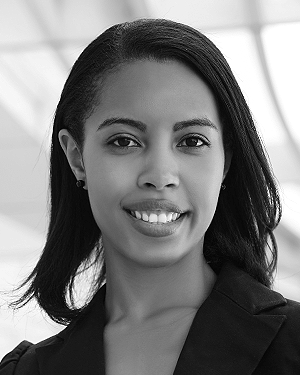
\includegraphics[width=1in,height=1.25in,clip,keepaspectratio]{a1.png}}]{First A. Author} (M'76--SM'81--F'87) and all authors may include
    biographies. Biographies are often not included in conference-related
    papers. This author became a Member (M) of IEEE in 1976, a Senior
    Member (SM) in 1981, and a Fellow (F) in 1987. The first paragraph may
    contain a place and/or date of birth (list place, then date). Next,
    the author's educational background is listed. The degrees should be
    listed with type of degree in what field, which institution, city,
    state, and country, and year the degree was earned. The author's major
    field of study should be lower-cased.

    The second paragraph uses the pronoun of the person (he or she) and not the
    author's last name. It lists military and work experience, including summer
    and fellowship jobs. Job titles are capitalized. The current job must have a
    location; previous positions may be listed
    without one. Information concerning previous publications may be included.
    Try not to list more than three books or published articles. The format for
    listing publishers of a book within the biography is: title of book
    (publisher name, year) similar to a reference. Current and previous research
    interests end the paragraph. The third paragraph begins with the author's
    title and last name (e.g., Dr.\ Smith, Prof.\ Jones, Mr.\ Kajor, Ms.\ Hunter).
    List any memberships in professional societies other than the IEEE. Finally,
    list any awards and work for IEEE committees and publications. If a
    photograph is provided, it should be of good quality, and
    professional-looking. Following are two examples of an author's biography.
\end{IEEEbiography}

\begin{IEEEbiography}[{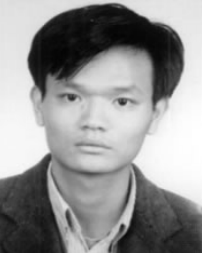
\includegraphics[width=1in,height=1.25in,clip,keepaspectratio]{a2.png}}]{Second B. Author} was born in Greenwich Village, New York, NY, USA in
    1977. He received the B.S. and M.S. degrees in aerospace engineering from
    the University of Virginia, Charlottesville, in 2001 and the Ph.D. degree in
    mechanical engineering from Drexel University, Philadelphia, PA, in 2008.

    From 2001 to 2004, he was a Research Assistant with the Princeton Plasma
    Physics Laboratory. Since 2009, he has been an Assistant Professor with the
    Mechanical Engineering Department, Texas A{\&}M University, College Station.
    He is the author of three books, more than 150 articles, and more than 70
    inventions. His research interests include high-pressure and high-density
    nonthermal plasma discharge processes and applications, microscale plasma
    discharges, discharges in liquids, spectroscopic diagnostics, plasma
    propulsion, and innovation plasma applications. He is an Associate Editor of
    the journal \emph{Earth, Moon, Planets}, and holds two patents.

    Dr. Author was a recipient of the International Association of Geomagnetism
    and Aeronomy Young Scientist Award for Excellence in 2008, and the IEEE
    Electromagnetic Compatibility Society Best Symposium Paper Award in 2011.
\end{IEEEbiography}

\begin{IEEEbiography}[{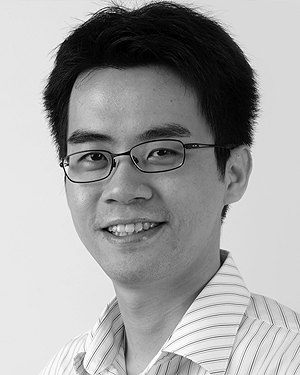
\includegraphics[width=1in,height=1.25in,clip,keepaspectratio]{a3.png}}]{Third C. Author, Jr.} (M'87) received the B.S. degree in mechanical
    engineering from National Chung Cheng University, Chiayi, Taiwan, in 2004
    and the M.S. degree in mechanical engineering from National Tsing Hua
    University, Hsinchu, Taiwan, in 2006. He is currently pursuing the Ph.D.
    degree in mechanical engineering at Texas A{\&}M University, College
    Station, TX, USA.

    From 2008 to 2009, he was a Research Assistant with the Institute of
    Physics, Academia Sinica, Tapei, Taiwan. His research interest includes the
    development of surface processing and biological/medical treatment
    techniques using nonthermal atmospheric pressure plasmas, fundamental study
    of plasma sources, and fabrication of micro- or nanostructured surfaces.

    Mr. Author's awards and honors include the Frew Fellowship (Australian
    Academy of Science), the I. I. Rabi Prize (APS), the European Frequency and
    Time Forum Award, the Carl Zeiss Research Award, the William F. Meggers
    Award and the Adolph Lomb Medal (OSA).
\end{IEEEbiography}

\EOD

\end{document}
